% topic: algorithms
\question จากตารางรหัสมอร์ส (Morse code) ด้านล่าง ถ้ารหัสมอร์สจากต้นทาง คือ 
\begin{verbatim}
    .... . .-.. .--.
\end{verbatim}
\begin{center}
    % เมื่อใช้งานจริงให้เปลี่ยนบรรทัดล่างนี้เป็นบรรทัดเรียกรูปภาพ เช่น: \includegraphics[width=0.35\textwidth]{image1.png}
    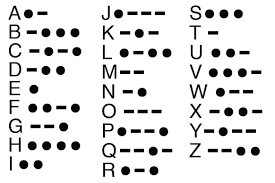
\includegraphics[width=0.35\textwidth]{morse_code_table.png}
\end{center} 
สามารถถอดความได้เป็นคำว่าอะไร
\newline
\choiceshorizontal{SELL}{HELLO}{HEAP}{HELP}
% answer: 4